\documentclass{beamer}
\usepackage[brazilian]{babel}
\usepackage[utf8]{inputenc}
\usepackage{calc}
\usepackage[absolute,overlay]{textpos}
\mode<presentation>{\usetheme{tud}}

\title[JEWEL]{JEWEL}
%\subtitle
\institute[HEPIC-Instituto de Física]{HEPIC-Instituto de Física}
\author{Fabio Canedo}
\date{\today}

% Insert frame before each subsection (requires 2 latex runs)
\AtBeginSubsection[] {
	\begin{frame}<beamer>\frametitle{\titleSubsec}
		\tableofcontents[currentsection,currentsubsection]  % Generation of the Table of Contents
	\end{frame}
}
% Define the title of each inserted pre-subsection frame
\newcommand*\titleSubsec{Content}
% Define the title of the "Table of Contents" frame
\newcommand*\titleTOC{Content}

% define a symbol which can be removed if you don't need it
\newcommand{\field}[1]{\mathbb{#1}}
\newcommand{\Zset}{\field{Z}}

\begin{document}

{
% remove the next line if you don't want a background image
\usebackgroundtemplate{}%
\setbeamertemplate{footline}{\usebeamertemplate*{minimal footline}}
\frame{\titlepage}
}

{\setbeamertemplate{footline}{\usebeamertemplate*{minimal footline}}
\begin{frame}\frametitle{\titleTOC}
	\tableofcontents
\end{frame}
}

\section{Quick Review}
\subsection{Something to think here}

\begin{frame}\frametitle{Something to think here}
        So far, I have developed a simulation in the following conditions
        \begin{itemize}
        \item JEWEL in its standard form;
        \item JEWEL with TRENTo initial conditions;
        \item JEWEL coupled with v-USPhyrdo simulations;
        \end{itemize}
        \begin{minipage}{1.0\textwidth}
		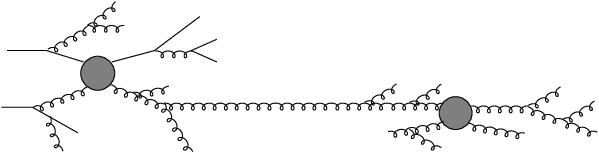
\includegraphics[scale=0.5]{images/feynman.png}        
        \end{minipage}
\end{frame}

\subsection{Observables chosen}
\begin{frame}\frametitle{Observables chosen}
	The observables chosen to be calculated are the following:
	\begin{itemize}
	\item $v_2^{ch jet}$;
	\pause
	\item \emph{girth};
	\pause
	\item \emph{grooming};
	\pause
	\item LeSub;
	\pause
	\item dispersion;
	\pause
	\item jet mass;
	\end{itemize}
\end{frame}

\subsection{Physics of JEWEL}

\begin{frame}\frametitle{Physics of JEWEL}
	The use of perturbative approach is dealt with by making use of a probabilistic interpretation
	of the Sudakov form factor:
	\begin{equation}
	S_a(t_h,t_c) = \exp \left\{ -\int_{t_c}^{t_h} \frac{dt}{t} \int_{z_{min}}^{z_{max}} dz \sum_b \frac{\alpha(k_{\bot}^2)}{2\pi} \hat{P}_{ab}(z) \right\}
	\end{equation}
	\pause
	Wich means we can take it as the probability that a parton $a$ emites no resolvable radiation
	between the scales $t_c$ and $t_h$.
\end{frame}

\begin{frame}\frametitle{Physics of JEWEL}
	The Sudakov form factor is used to perform the evolution by enforcing radiation until the
	parton reaches the $t_c$ \textit{cut-off}.
	\\ \pause
	Besides that, the medium, seen as a collection of scattering centers by the parton, also has
	the probability of interaction.
	\\ \pause
	This probability is given by the regular cross-section of a $2 \rightarrow 2$ process,given by:
	\begin{equation}
	\sigma_i(E,T)=\int_{0}^{|\hat{t}|_{max}(E,T)}d|\hat{t}|\int_{x_{min}(|\hat{t}|)}^{x_{max}(|\hat{t}|)} dx \sum_{j \in \{ q,\overline{q},g\}} f_{j}^{i}(x,\hat{t})\frac{\mathrm{d}\sigma}{\mathrm{d}\hat{t}}(x\hat{s},|\hat{t}|)
	\end{equation}
\end{frame}

\section{Medium Model}
\subsection{Initial Conditions}

\begin{frame}\frametitle{Initial Conditions}
	The model employed by JEWEL is a variant of Bjorken model that
	approachs the initial contitions by the definition of the nuclear thickness 
	function:
	\begin{equation}
	T(x,y) = \int dz \rho(x,y,z)
	\end{equation}
\end{frame}

\begin{frame}\frametitle{Initial Conditions}
	The nuclear thickness functions are then used to define a reduced thickness by:
	\begin{equation}
	\begin{split}
	n(b,x,y) &= T_A(x-\frac{b}{2},y) \left( 1-\exp\left( \sigma_{NN} T_B(x+\frac{b}{2},y) \right) \right) \\
	&+ T_B(x+\frac{b}{2},y) \left( 1-\exp\left( \sigma_{NN} T_A(x-\frac{b}{2},y) \right) \right)
	\end{split}
	\end{equation}
	Where $\sigma_{NN}$ is the nuclear cross-section and $b$ is the impact parameter.
\end{frame}

\begin{frame}\frametitle{Initial Conditions}
	This reduced thickness is then applied to take a map of the initial energy density:
	\begin{equation}
	\epsilon(x,y,b,\tau_i) = \epsilon_i \frac{n_{part}(x,y,b)}{<n_{part}>(b=0)}
	\end{equation}
	Where $<n_{part}>(b=0) \approx \frac{2 A}{\pi R_A}$.
\end{frame}

\begin{frame}\frametitle{Initial Conditions}
	The value of $\epsilon_i$ is determined by an initial temperature given as a parameter to
	JEWEL. This translation is made through the use of the relation $\epsilon_i \propto T_i^4$.
\end{frame}

\begin{frame}\frametitle{Initial Conditions}
	The new feature added in this work regarding the initial conditions is also the
	vertex production of the high energy partons. Here the production vertex is randomly
	chosen from a 2D spatial distribuition function proportional to $T^4$. This is necessary
	if one desires to have consistency with arbitrary entropy distributions.
\end{frame}

\subsection{Medium Evolution}

\begin{frame}\frametitle{Medium Evolution}
	In the case of v-USPhydro, the evolution is given entirely by a hydro simulation.
	Otherwise(TRENTo and Glauber), the medium evolution is performed analytically by use of:
	\begin{equation}
	\epsilon(x,y,b,\tau) = \epsilon_i (x,y,b,\tau_i) \left( \frac{\tau}{\tau_i} \right)^{-\frac{4}{3}}
	\end{equation}
	\pause
	This that the temperature evolves according to:
	\begin{equation}
	T(x,y,b,\tau) \propto \epsilon(x,y,b,\tau_i)^{1/4} \left( \frac{\tau}{\tau_i} \right)^{-\frac{4}{3}}
	\end{equation}
\end{frame}

\section{Jet Observables}
\subsection{JetAlgorithms}

\begin{frame}\frametitle{Jet Algorithms}
	Today, the main type of algorithm to cluster particles from a given event into jets,
	thus defining a jet, are the sequential recombination algorithms. They define a distance
	functions between particles:
	\pause
	\begin{equation}
	d_{ij} = \min(p_{ti}^{2p},p_{tj}^{2p}) \frac{\Delta R_{ij}^2}{R^2}
	\end{equation}
	\pause
	Then a process of iteration is realized, where the particles with minimum $d_{ij}$ are
	combined to form the given jets.
\end{frame}

\begin{frame}\frametitle{Jet Algorithms}
	Once the jets are found, one class of the possible observables are the jet shape observables.
	\pause
	\\
	These reflect mush of the evolution that occurs in the jet formation, as well as
	the process of hadronization.
\end{frame}

\subsection{SoftDrop Procedure}

\begin{frame}\frametitle{SoftDrop Procedure}
	One form of extracting information about jet shape is through the SoftDrop Procedure.
	\pause
	\\
	This is done by undoing the last step of the jet recombination.
	\pause
	\\
	The SoftDrop condition is:
	\begin{equation}
	\frac{\min(p_{T1},p_{T2})}{p_{T1}+p_{T2}} > z_{cut} \left(\frac{\Delta R_{12}}{R_0}\right)^{\beta}
	\end{equation}
\end{frame}

\begin{frame}\frametitle{SoftDrop Procedure}
	Once the condition has been applied, the quantity:
	\begin{equation}
	\frac{\min(p_{T1},p_{T2})}{p_{T1}+p_{T2}}
	\end{equation}
	Reflects an observable that is usually related to the first splitting of the parent parton.
	\pause
	\\
	This can be seen in the results of the fact that they follow the Altarelli-Parisi splitting
	functions.
\end{frame}

\subsection{Angularity}

\begin{frame}\frametitle{Angularity}
	This variable is defined as:
	\begin{equation}
		g = \frac{\sum_{i} p_i^{T} \Delta R_i}{p_{J}^{T}}
	\end{equation}
	It measures how spread out is a jet.
\end{frame}

\subsection{$p^T_{D}$}

\begin{frame}\frametitle{$p^T_{D}$}
	This variable is defined as:
	\begin{equation}
		p^T_{D} = \frac{\sqrt{\sum_{i} {p_i^{T}}^2}}{p_{J}^{T}}
	\end{equation}
	It measures the \emph{hardness} of a jet. It is closer to one if one or a few
	particles carry most of the jet momenta.
\end{frame}

\subsection{$x_J$}

\begin{frame}\frametitle{$x_J$}
	The $x_J$ variable is simply the ratio of the subleading jet transverse momentum to the
	leading jet transverse momentum. It is a \emph{traditional} jet quenching variable. 
	The usual interpretation is that, quite often a pair of partons will traverse different
	path lengths, resulting in different quenching experienced by these partons. This
	variable attempts to quantify this phenomena.
\end{frame}

\subsection{Jet $v_2$}

\begin{frame}\frametitle{Jet $v_2$}
	This variable is also related to path length dependency. It is the second harmonic
	contribution to the jet medium angular correlation. In central collisions, it is also
	an indicative of fluctuating initial conditions.
\end{frame}

\section{Preliminary JEWEL Results}

\subsection{Preliminary JEWEL results of the current work}

\begin{frame}\frametitle{Current Work}
	In this work, currently four different types of simulations were performed. The first is JEWEL
	on its default mode. The other ones had a modification such that a code was
	inserted in order to allow it to read an external temperature profile on a given grid. The
	temperature on arbitrary points are given by a bicubic interpolation. On this mode we had
	the following:
	\begin{itemize}
		\item JEWEL+PYTHIA default;
		\pause
		\item JEWEL+PYTHIA with TRENTo initial conditions;
		\pause
		\item JEWEL+PYTHIA+v-USPhydro;
	\end{itemize}
\end{frame}

\begin{frame}\frametitle{Current Work}
	\begin{minipage}{1\textwidth}
	The first results for the jet transverse momentum are given here:
    \end{minipage}
    \begin{columns}
    \begin{column}{0.5\textwidth}
	\begin{minipage}[l]{0.5\textwidth}
	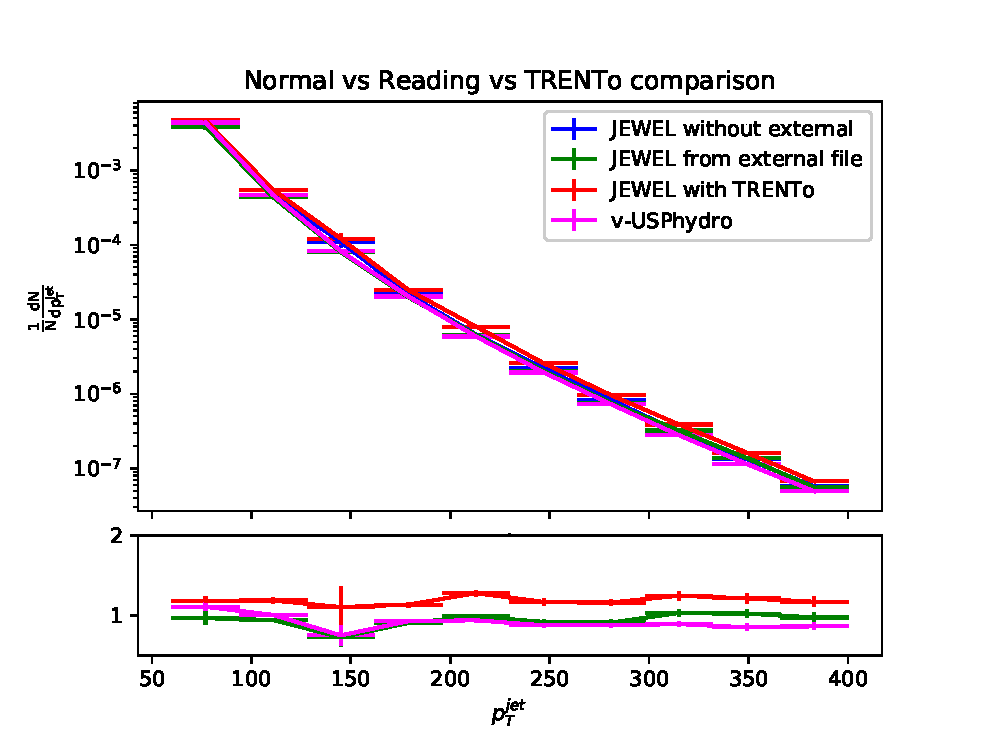
\includegraphics[scale=0.4]{images/pt_cheking_consistency.eps}
	\end{minipage}
	\end{column}
    \begin{column}{0.4\textwidth}
	\begin{minipage}[r]{1\textwidth}
	These results represent a well predicted observable and therefore represent a good
	check on to whether the simulations are consistent.
	\end{minipage}
	\end{column}
	\end{columns}
\end{frame}

\begin{frame}\frametitle{Current Work}
	\begin{minipage}{1\textwidth}
	The first results for the $p_{T}^{D}$ momentum are given here:
    \end{minipage}
    \begin{columns}
    \begin{column}{0.5\textwidth}
	\begin{minipage}[l]{0.5\textwidth}
	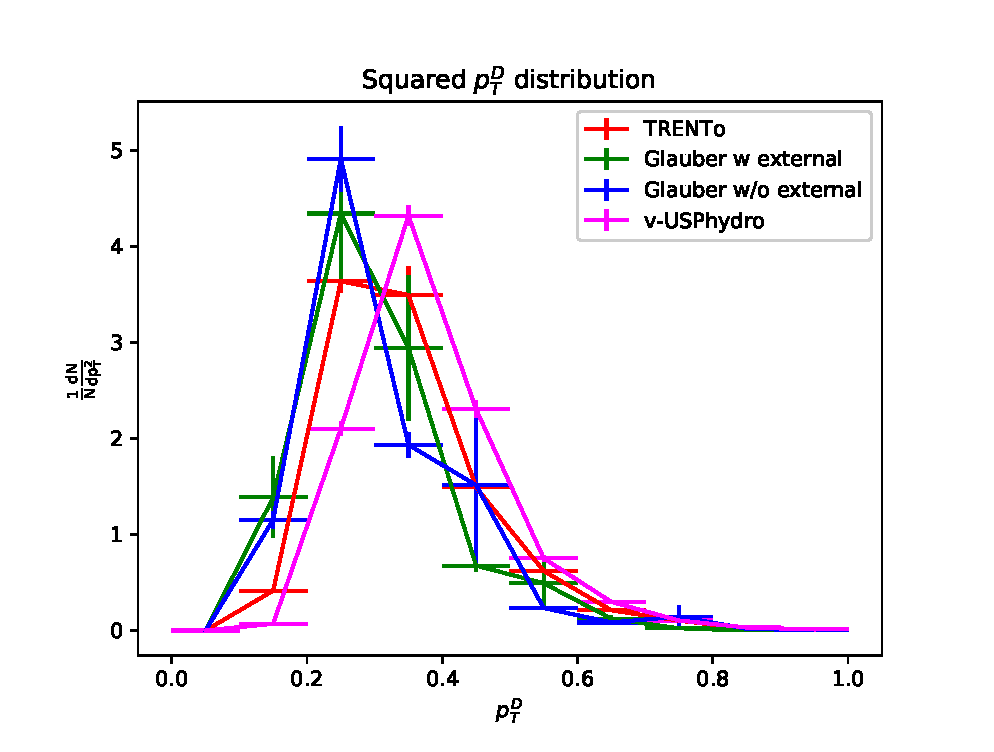
\includegraphics[scale=0.4]{images/Squared.eps}
	\end{minipage}
	\end{column}
    \begin{column}{0.4\textwidth}
	\begin{minipage}[r]{1\textwidth}
	
	\end{minipage}
	\end{column}
	\end{columns}
\end{frame}

\begin{frame}\frametitle{Current Work}
	\begin{minipage}{1\textwidth}
	The first results for the \emph{girth} momentum are given here:
    \end{minipage}
    \begin{columns}
    \begin{column}{0.5\textwidth}
	\begin{minipage}[l]{0.5\textwidth}
	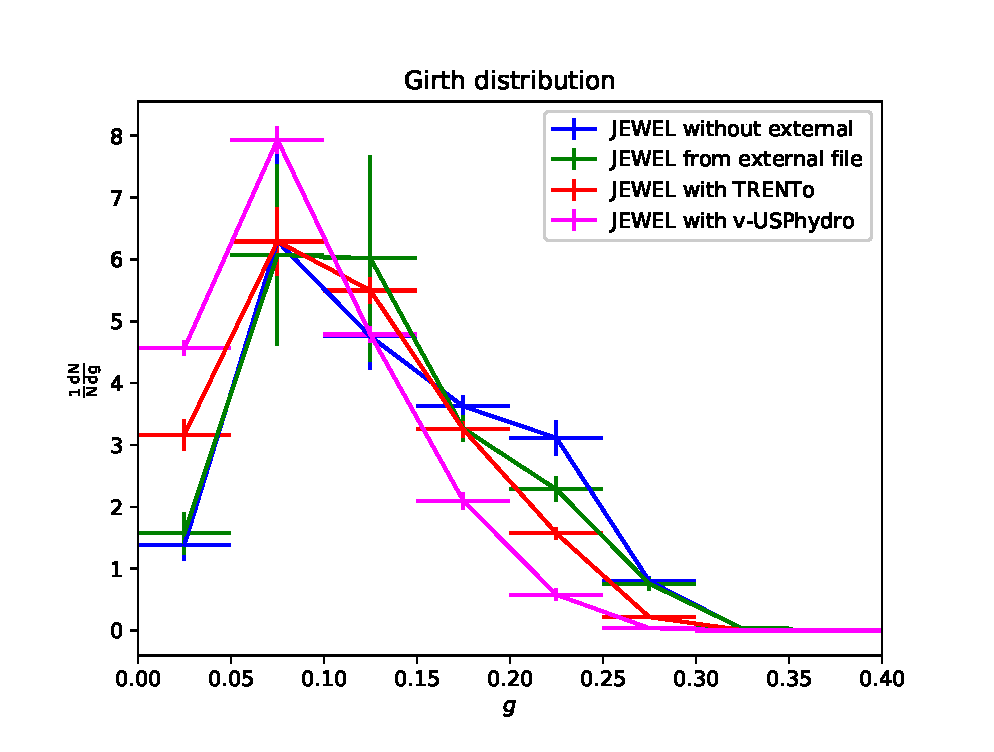
\includegraphics[scale=0.4]{images/Angularity.eps}
	\end{minipage}
	\end{column}
    \begin{column}{0.4\textwidth}
	\begin{minipage}[r]{1\textwidth}
	
	\end{minipage}
	\end{column}
	\end{columns}
\end{frame}

\begin{frame}\frametitle{Current Work}
	\begin{minipage}{1\textwidth}
	The first results for the jet $v_2$ momentum are given here:
    \end{minipage}
    \begin{columns}
    \begin{column}{0.5\textwidth}
	\begin{minipage}[l]{0.5\textwidth}
	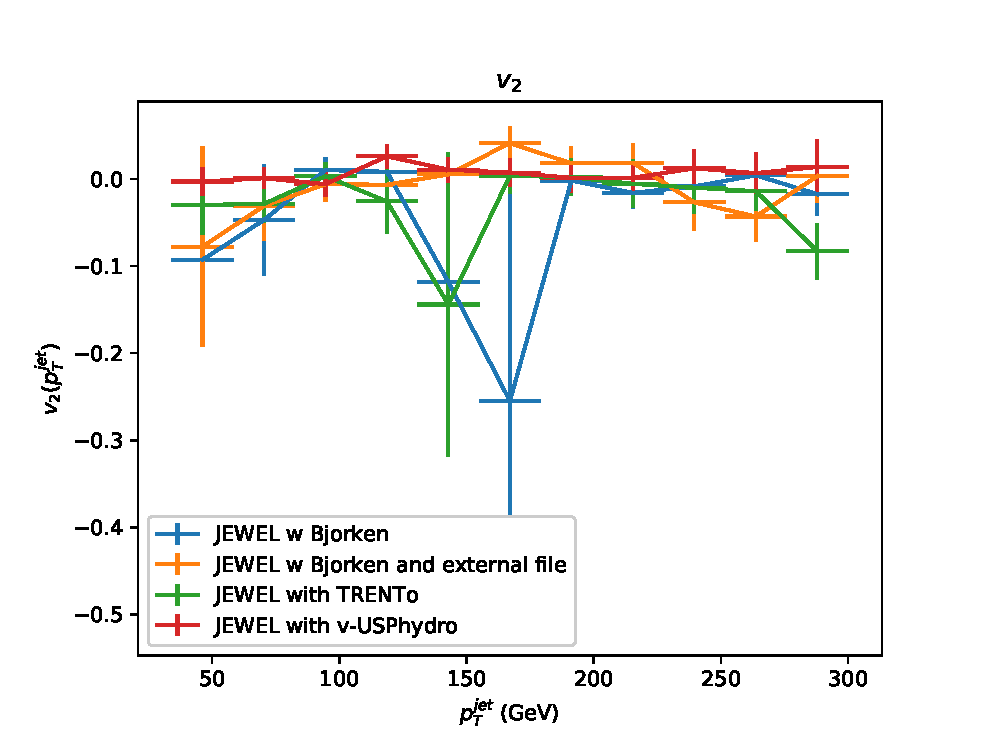
\includegraphics[scale=0.4]{images/v2.eps}
	\end{minipage}
	\end{column}
    \begin{column}{0.4\textwidth}
	\begin{minipage}[r]{1\textwidth}
	
	\end{minipage}
	\end{column}
	\end{columns}
\end{frame}

\begin{frame}\frametitle{Current Work}
	\begin{minipage}{1\textwidth}
	The first results for the \emph{grooming} are given here:
    \end{minipage}
    \begin{columns}
    \begin{column}{0.5\textwidth}
	\begin{minipage}[l]{0.5\textwidth}
	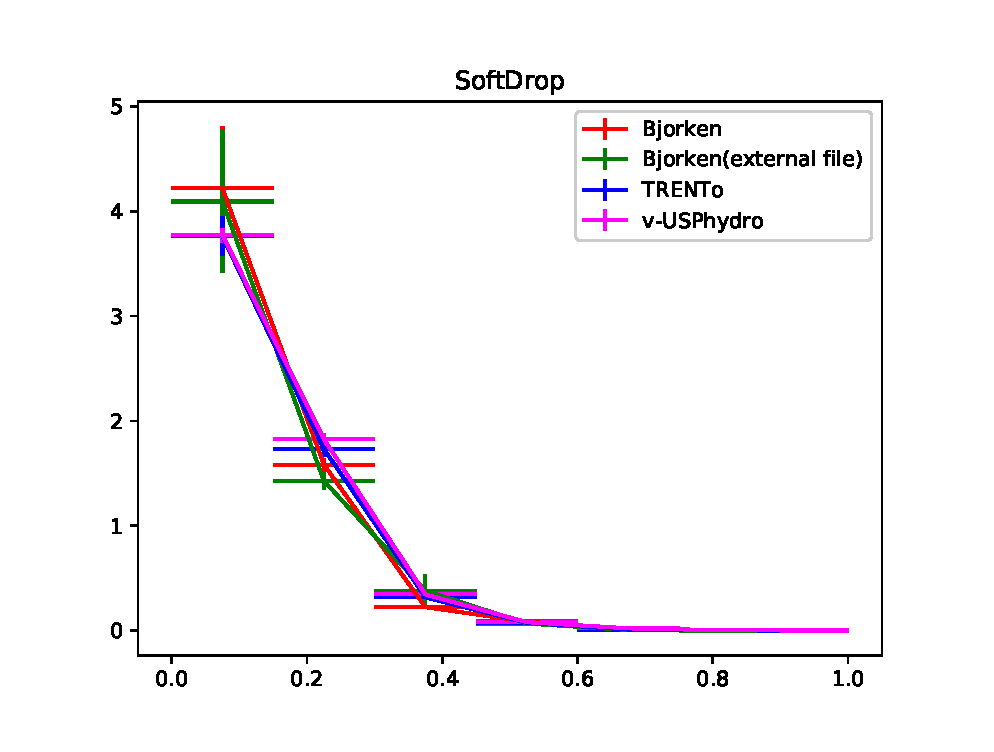
\includegraphics[scale=0.4]{images/softdrop.eps}
	\end{minipage}
	\end{column}
    \begin{column}{0.4\textwidth}
	\begin{minipage}[r]{1\textwidth}
	
	\end{minipage}
	\end{column}
	\end{columns}
\end{frame}

\begin{frame}\frametitle{Current Work}
	\begin{minipage}{1\textwidth}
	The first results for the LeSub are given here:
    \end{minipage}
    \begin{columns}
    \begin{column}{0.5\textwidth}
	\begin{minipage}[l]{0.5\textwidth}
	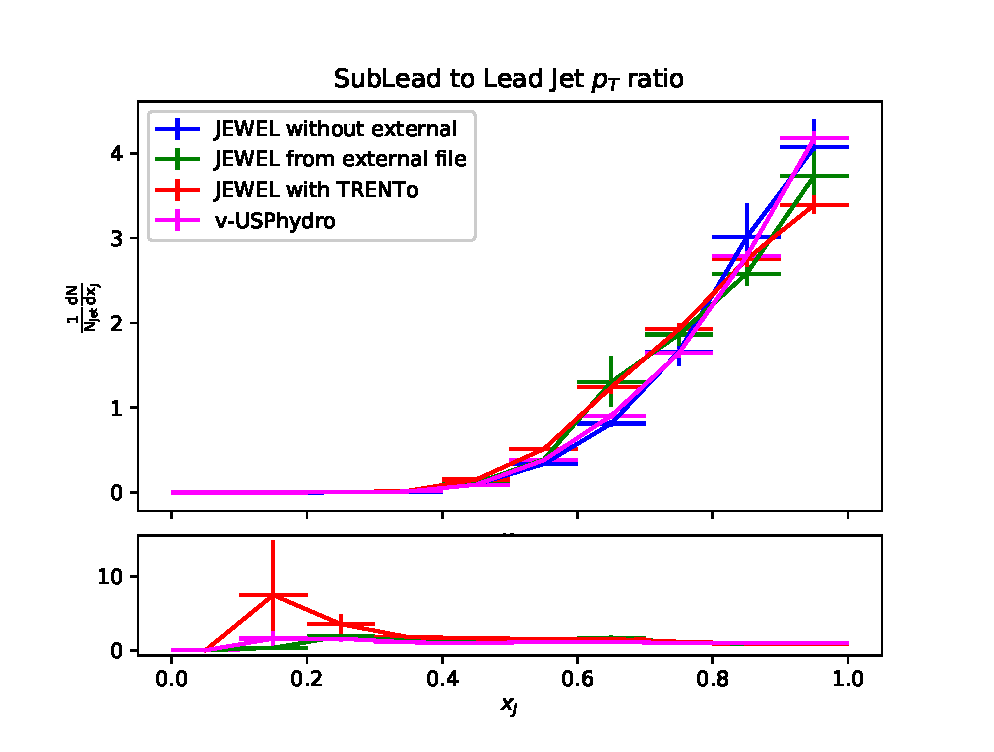
\includegraphics[scale=0.4]{images/LeadToSub.eps}
	\end{minipage}
	\end{column}
    \begin{column}{0.4\textwidth}
	\begin{minipage}[r]{1\textwidth}
	
	\end{minipage}
	\end{column}
	\end{columns}
\end{frame}

\begin{frame}\frametitle{Current Work}
	\begin{minipage}{1\textwidth}
	The first results for the jet mass are given here:
    \end{minipage}
    \begin{columns}
    \begin{column}{0.5\textwidth}
	\begin{minipage}[l]{0.5\textwidth}
	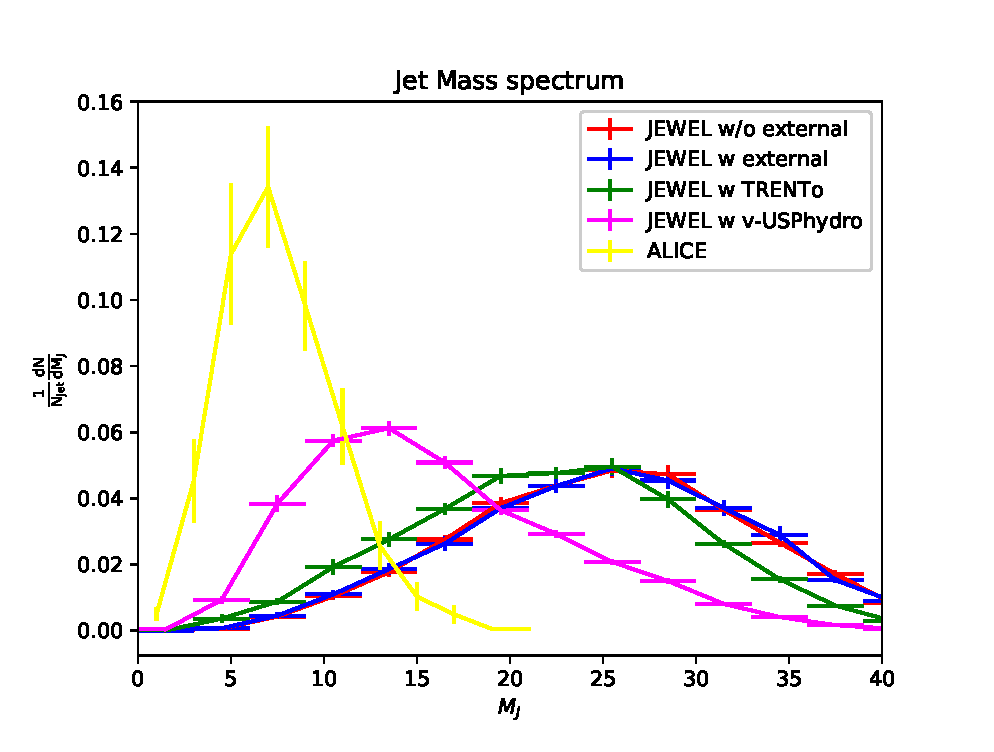
\includegraphics[scale=0.4]{images/Mass.eps}
	\end{minipage}
	\end{column}
    \begin{column}{0.4\textwidth}
	\begin{minipage}[r]{1\textwidth}
	
	\end{minipage}
	\end{column}
	\end{columns}
\end{frame}

\end{document}
